\documentclass[11pt]{article}

\usepackage{fullpage}
\usepackage{graphicx}

\begin{document}

\title{Final Report}
\author{Ashton Choy, Rohan Pandit, Clara Stoddart, Ian Ren }
\date{June 2020}

\maketitle

Building our assembler and working on our own extension has taught us a lot about programming in C, communicating with others, and making independent decisions regarding implementation and design. Here we reflect on some of the difficulties we faced, what we gained from this project, and how we designed and structured our assembler and extension.

\section*{Assembler Structure}
To structure the assembler, we created two utility directories in src: global\_utils and assembler\_utils. For each .c file we defined a corresponding header file. These header files contain function declarations and definitions of constants, structures and enums, which are all used in the header's respective .c file.
We created the global\_utils directory for files used in both the emulator and assembler. We put the files from binary\_utils, originally made for the emulator, into global\_utils, our assembly files also manipulate binary numbers. Additionally, we added an error handling .h file containing useful macros for frequent actions such as checking for memory allocation failures / string validity. In our implementation of the assembler we encode the instructions over two passes. The first populates the symbol table with labels and their associated memory addresses. We also populate the symbol table with mnemonics as strings, eg. "add", "mov", etc.,  paired with their corresponding opcode enum type. This allows us to easily associate an integer value with each instruction type. Our assembler\_utils directory contains a file hashmap.c which allows us to create a hashmap data structure which we use to represent the symbol table. The second pass uses the tokenizer.c file to "tokenize" and breakdown each ARM instruction into fields such as opcode, registers, and much more, returning them as part of a INSTR\_TOKENS structure. The encode.c file contains specific encode functions for each instruction type. These take in an INSTR\_TOKENS structure and return the machine code representation of the ARM instruction. For our encode single data transfer function we created a file sdtconstants.c; this contains functions to create and free our structure SDT\_CONSTANTS. This structure, defined in sdtconstants.h, stores and tracks the number of constants given by load instructions. We use this structure to work out the correct offset when encoding load instructions, and to keep track of any immediate values to be written to the end of the binary output file as described in the spec.

\section*{Extension description}

For our extension we decided to make an IDE for writing assembly programs based on the suggestions given in the specification. We felt this could be a useful tool that would also apply the emulator and assembler that we had already made. As making a suitable GUI seemed difficult and time-consuming to achieve in C we decided to instead focus on a command-line type of interface that is intuitive and useful for the user. To establish the basic framework we created an enum for the top level commands such as "help", "quit" and "clear". There is a "info" command that gives information about what the different commands do as well as explain the format for writing different assembly instructions. To parse the user input Rohan decided to use spaces-separated arguments. The input string is read from the user and tokenized into an array of argument strings. The first token is used to determine the command. Each command has its own function that takes the current state of the IDE in an \textit{Editor} struct. Originally we were handling commands using a switch statement but later on we decided to use function pointers to handle each command. Then we created an array of strings to store the text that the user types. Using the "write" command, the program reads lines inputted by the user into the array which can later be displayed using the "display" command along with the line numbers.

Later on we all worked on how to run the program line by line as in a debugger instead of simply running till it halts. To do this we had to slightly change the design of emulate.c. We encapsulated one cycle of the pipeline into its own function which could be repeatedly called instead of executing the program in one loop. This allowed us to execute one instruction at a time. Later on we had some difficulty in executing branch instructions and tracking the current line number. To resolve this issue we noticed that the pipelineCycle should be called until the pipeline is ready to execute an instruction after branching to a label or address. We also added support for inline comments, basic syntax checking, syntax highlighting and displaying the execution time of the program. The state of the machine can be printed at any time using the "state" command. The user can "export" any code they have written to a text file, or "load" text in from an existing file.

After we could execute a program one instruction at a time using the "next" command we made a "finish" command that would run the program from the current point till the end. To ease editing text we implemented insert and delete functions to increase efficiency. We also included an "append" command to add text at the end of a line (to add a comment for example).

Our program also allows the user to set, disable and utilise breakpoints at desired lines in their assembly code, in similar fashion to popular debuggers such as GDB. The continue command stops execution when it reaches the next breakpoint. The IDE can also calculate the execution time of the assembly program using the "run all" command.

When testing one of the programs we noticed that the program never finished due to an error in the code and as a result we had to close the entire IDE and rerun it. This inspired us to create a fail-safe to avoid this kind of a situation. Hence we decided to set a limit to the number of times pipelineCycle can be called.

Although not as interactive as modern IDEs' graphics we still feel that for the purposes of running assembly programs our attempt can prove to be quite useful and intuitive for people to understand.
Originally we wanted to be able to dynamically edit and highlight code and syntax errors however that was hard to achieve in such a short time frame.


\section*{Testing our implementation}
We frequently ran the given test suite while coding our implementation, comparing the expected output with the actual output produced by our program to see where we went wrong. Once we spotted a difference, we would use CLion's debugger and go through our program line by line to see what was causing the issue. This proved to be effective for the most part, however for some bugs involving memory allocation we found it better to use GDB as we could easily disable address space randomization which caused our program to occasionally (and misleadingly) work fine in CLion. We found that the provided test suite was varied enough in its testing that we did not need to add any test cases of our own.

Due to the command-line interface nature of our extension, it was hard to create a suitable test suite that would be able to navigate our program. As our extension is an assembly IDE, we found that the best way to see if it was working as intended was to load in the existing .s assembly files provided as part of the college's test suite, and see if our extension's commands gave the desired results / outputs according to what each assembly program should have done.

To test additional features of our extension, such as being able to time out if it's executing a program that is too long, we purposefully wrote instructions that would result in an infinite loop.

\section*{Group reflection}

This project has been an interesting and enriching experience for all of us. We have developed our C programming skills, and our ability to effectively communicate with others. We have become more comfortable using a range of tools introduced to us this year, including GDB, Makefiles and Valgrind.

We have had several new experiences, including debugging large programs, working with a shared git repo, and programming in a group for the first time. Since our group was not entirely premade, we experienced getting to know new people and their work styles. This was a very valuable experience, since in future careers we may also be programming with people we have not met before, or do not know very well.

One difficulty we faced was becoming more dependent on GitLab, and learning the "Git workflow" - we had to learn together about merging, pulling and committing without negatively impacting code someone else had written. Although difficult, we know this is an essential skill for the future.

Another difficulty was the early design and implementation decisions we had to make at the start of building the emulator, assembler and the extension. These were difficult to agree on. The discussions we had at these early stages taught us all a lot, about communication, compromise and designing programs.

Since we were carrying out this project remotely, and did not have access to the labs, we could not easily compare our progress with other groups. We had no idea if we were making the right decisions, or working at the right pace. This was intimidating, but perhaps also a blessing: it allowed us to become more independent in our coding practice, encouraging more self-study and learning from our own mistakes - important aspects of any learning process.

Overall, we feel that this project has been a very valuable (and enjoyable!) experience, and we look forward to more of this type of work in the coming academic year.

\section*{Individual reflections}

\subsection*{Ian Ren}
Before beginning the project, I knew that I was not a very confident programmer but throughout the entire project, I always felt comfortable working with my team even though this has been the biggest and most difficult project I have ever worked on. I had previously studied and discussed programming with some of the other members before, so I had a good idea of where I fitted in, in terms of strengths and which types of problems I should work on.

I think the way we structured the workload and how we called almost every day allowed me to be much more productive than I would have been. If there was anything that I was struggling with, my team would be quick to respond and help. This went both ways, and the collaboration of ideas allowed us to progress quickly. However I believe our system was only effective because of our team’s personalities. I think that what system my next group will choose to work in should be flexible and based on the strengths and weaknesses of the team members. In addition, I believe the most important thing to maintain is lots of communication. Having everyone know exactly what and when things need to be done is paramount in avoiding confusion and keeping the project moving.

In the first DoCPA feedback, I received a rating of 4.67. I think this is accurate as it shows that I made an effort to contribute to the group and attend every meeting but there were a few occasions where I was confused with the problem at hand and was unable to provide useful contributions. I believe that as my ability improves so will my ability to contribute to a team.

\subsection*{Clara Stoddart}
Throughout this project I have learnt a lot, with regards to both programming in C and programming in a group.

I feel comfortable and at ease with my group mates, which makes offering ideas easier, and has made the project as a whole more enjoyable. We've all come to understand each other's strengths and weaknesses - for example, one of my weaknesses is with binary numbers. I find visualising shifts and bit masks difficult, hence I did not work on our bit manipulation files. Instead I worked on our main functions and file reading/writing logic, since for me writing these parts of the code was easier to understand.

Since we all rely on different editors and use different operating systems, being in a group allowed us to have access to different types of software and debuggers. For example, when we wanted to see all our variables more clearly we'd use the CLion debugger, which Ashton and Ian both use. However, when we had memory issues at the start of building our assembler, we relied more on the GDB debugger, which I use. We felt GDB was easier to use in this case since in our CLion debugger some memory issues did not appear. This was because the CLion debugger by default disables address space randomization. Since in GDB we could set "disable-randomization" off, GDB allowed us to pin down memory issues more easily. Hence the group project meant I got a lot more comfortable with using GDB, as well as learning more about memory layout and how different debuggers treat memory. Moreover, some test cases passed on one person's computer, but not everyone's, which alerted us to the fact that we had undefined behaviour. Had we not checked the tests on multiple people's computers, we may not have become aware of these bugs in our code.

In my first DocPA feedback, I received 4.67, which I feel indicates that I worked hard but could have done more to contribute, and this is something I should improve on. Overall, I feel that everyone made valuable contributions to our project and worked hard.

When working with a different type of people, I would like to maintain the ease of communication that I felt was present in my current group. Moreover, I hope that in my next group project I feel as comfortable expressing ideas and opinions as I did in this group project.


\subsection*{Rohan Pandit}
Originally I did not know which group I was going to be a part of. However when I was assigned to a group the other team mates soon contacted me so we could start discussing about the project from an early stage. Although working as part of a group remotely was a new process for us we were able to manage it fairly well. Everyone was very cooperative and considered all the suggestions that I gave so we were able to collaborate effectively and reach the targets we had set. Previously I didn't have much experience in using Git as part of a group however but we were able to write the code using an online IDE (repl.it) and then test the code locally. This enabled us to work at a faster rate because we could discuss our solutions before implementing them as well as notice errors or improvements.
In my first DocPA feedback I received a score of 5 so I am glad that I was beneficial for my group though my communication may not have been clear at times. By working as part of a group I was able to learn new things and think about problems from a different perspective.
Next time I work as part of a group I will make sure to use Git more effectively keep track of all the changes I make to the code and try to convey my ideas more clearly .


\subsection*{Ashton Choy}
I was anxious going into this C group project - we'd have to start from virtually no skeleton code, and finish with a working implementation of the longest specification we'd received from Imperial thus far; all in a C, a language we were only just getting to grips with. However, I can now say I have thoroughly enjoyed and learnt from the past few weeks of hard work. I think our group worked very well together, voice-calling almost every day when coding to ensure everyone is kept updated on each other's work. Everyone agreed that communication was key when working on such a large and rapidly evolving codebase, and I always felt like my opinions and ideas were welcomed, respected and acted upon by the group. Working with others also meant we could fill in for each other's weaknesses. The concepts of pointers and memory allocation are some things I personally struggled with while learning C, so during the coding process my other group members would help explain how to utilise these concepts correctly and effectively, and perhaps allow me to focus my attention more on other areas of the codebase where I could be more productive. Although I had not met all of my fellow group members prior to starting the project, I feel as though we've all become familiar with each other's styles of work, allowing us to complement each other well.

In the first DoCPA feedback I received a 4.67 rating, which reassured me that I had fit into the group well, but that there was also room for more contribution - I took this into consideration for the remainder of the project when working on the assembler and extension.

While our "call every day and code together" approach did prove effective for our group, I feel that future group projects may benefit from more independent coding from each member. Due to the nature of the current state of the world (with everyone in quarantine at home due to COVID-19) it was easy to arrange a common time for all members to call and collaborate, however in future this may be harder as people will have more commitments at conflicting times. Thus it is essential that a good "Git team workflow" is established - where members can each work in their own time, coordinating work so as to avoid any merge conflicts.
\newpage
\appendix
\section*{Appendix}

\begin{figure}[ht]
    \centering
    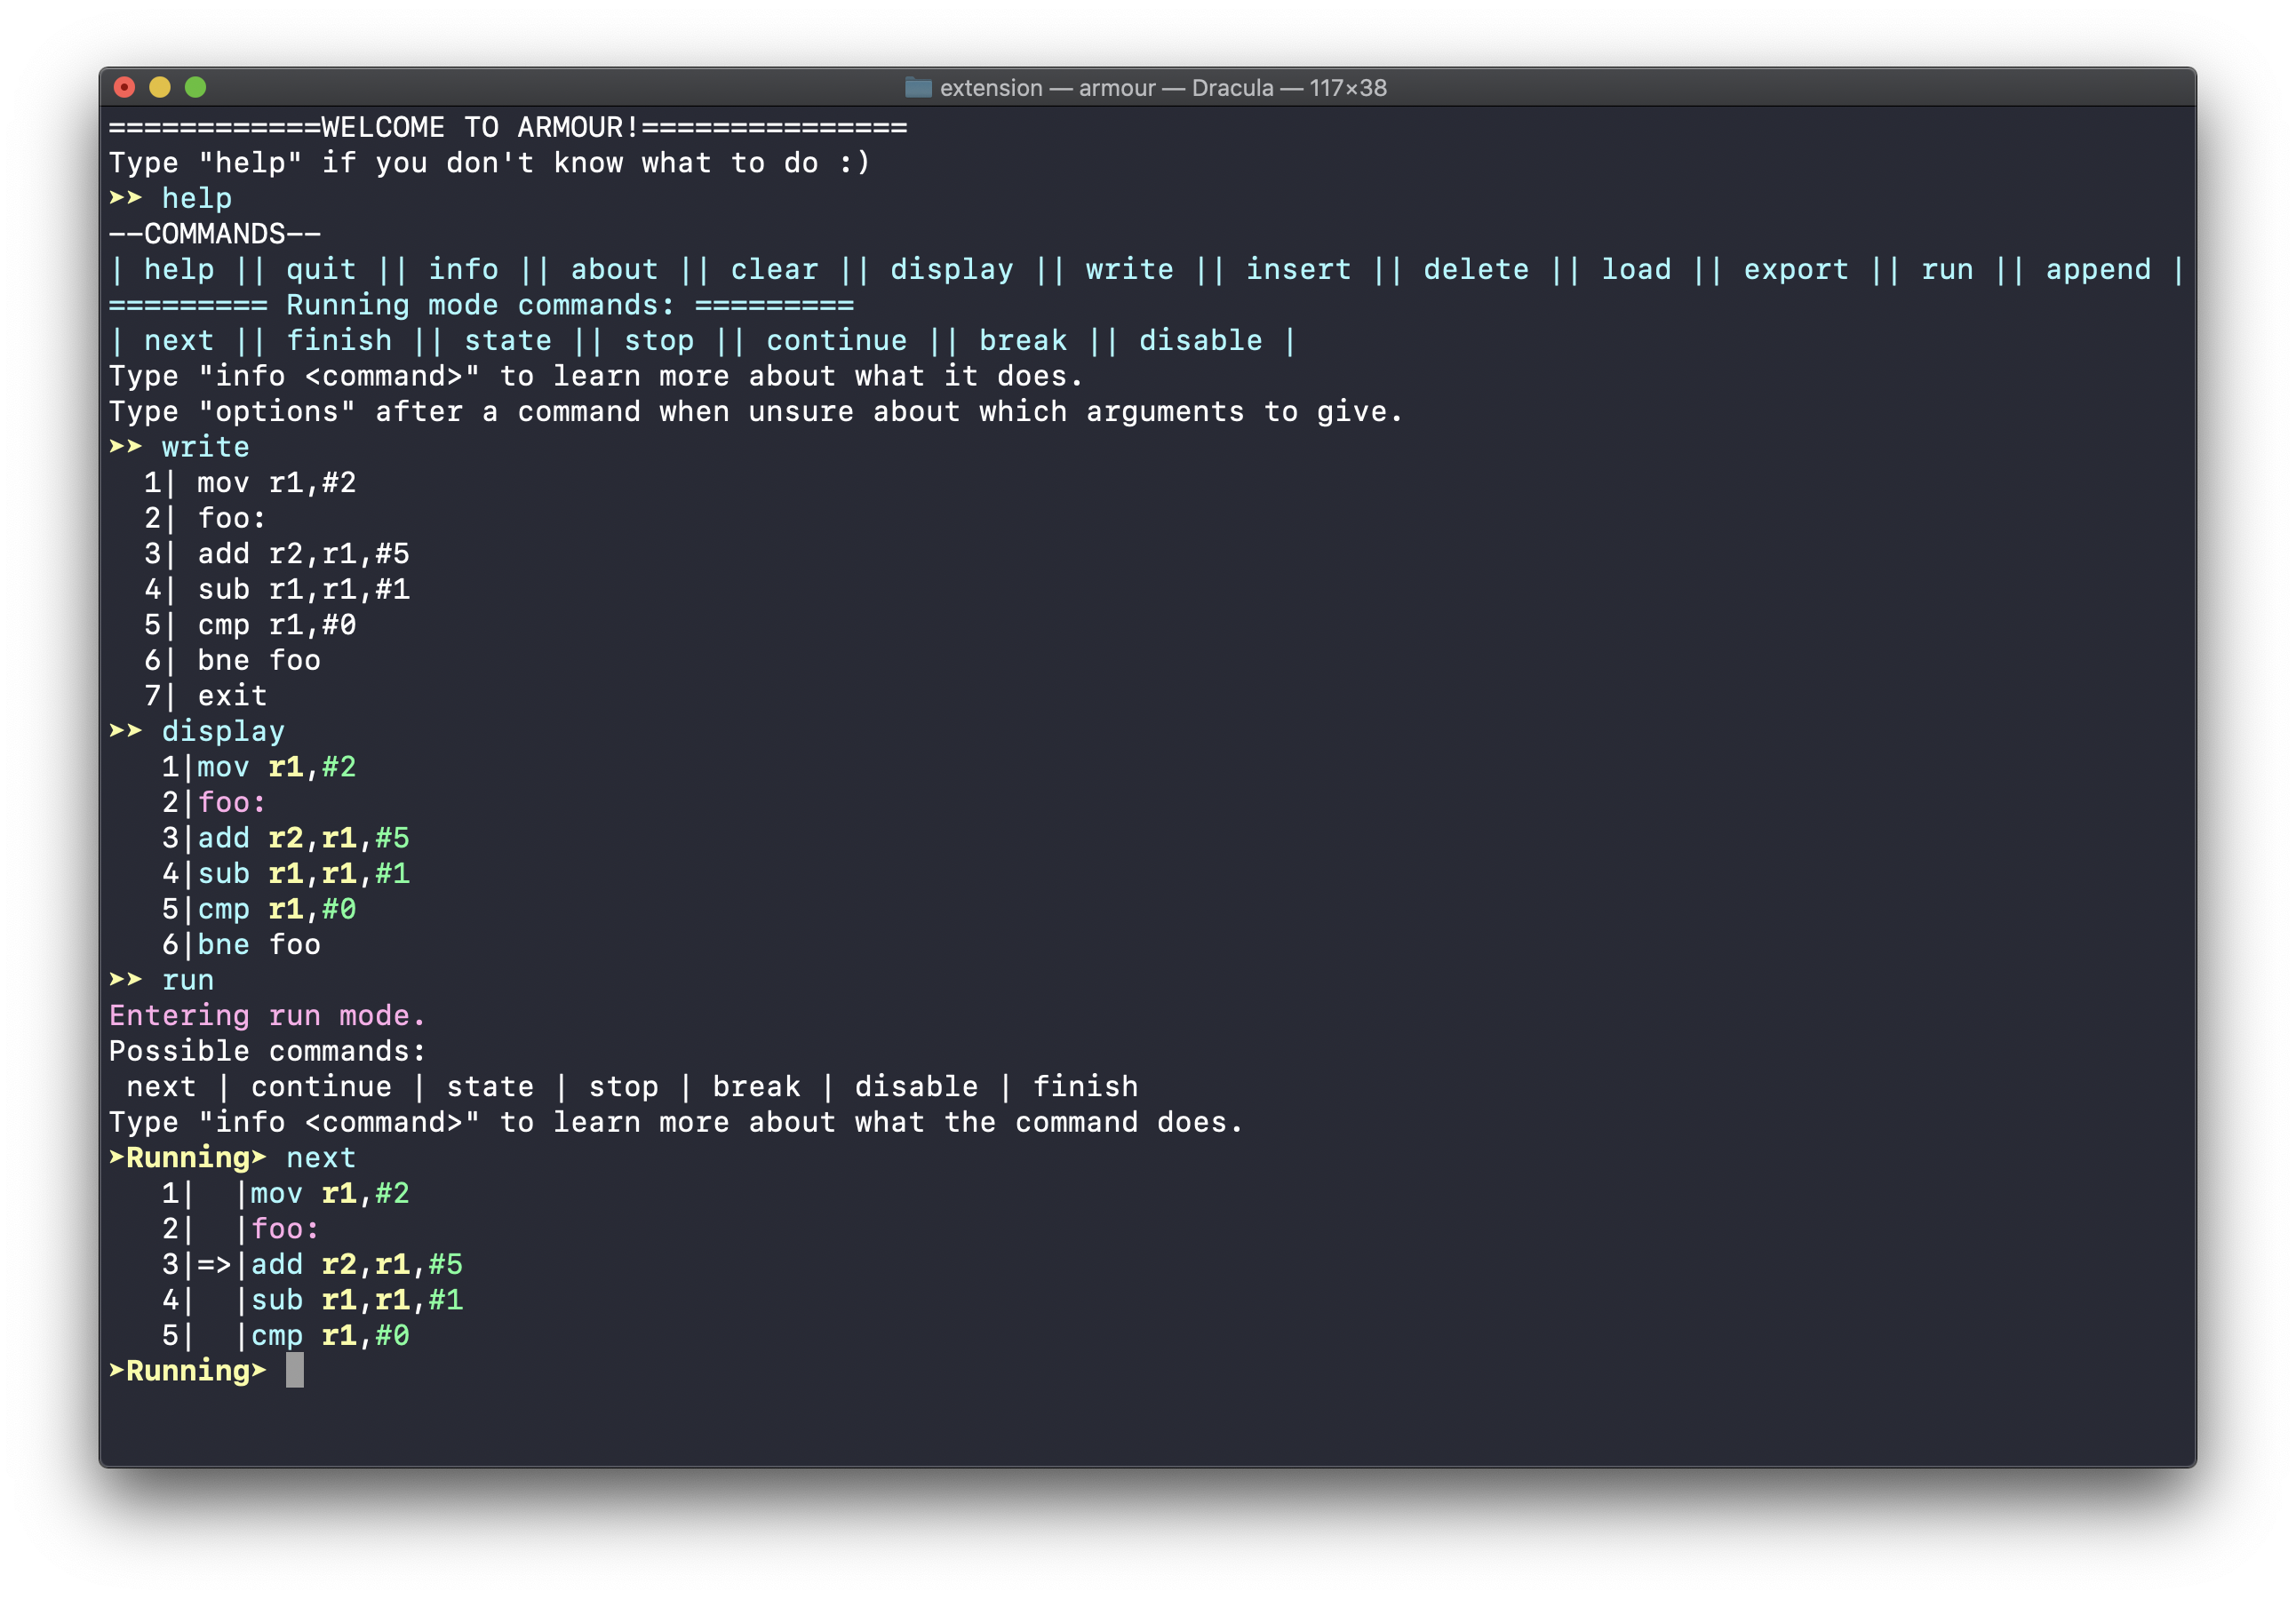
\includegraphics[scale = 0.3]{armour.png}
    \caption{An example of how our extension may be used.}
    \label{fig:my_label}
\end{figure}

\end{document}
